\documentclass[11pt]{article}

\usepackage[a4paper,margin=23mm]{geometry}
\usepackage[T1]{fontenc}
\usepackage[utf8]{inputenc}
\usepackage{amsmath,amssymb}
\usepackage{array}
\usepackage{booktabs}
\usepackage{enumitem}
\usepackage{longtable}
\usepackage{tabularx}
\usepackage{xcolor}
\usepackage{listings}
\usepackage{tikz}
\usetikzlibrary{arrows.meta,calc,fit,positioning,shapes.geometric}
\usepackage[hidelinks]{hyperref}

\setlength{\parindent}{0pt}
\setlength{\parskip}{0.55em}
\setlist{leftmargin=*,nosep}
\emergencystretch=3em
\renewcommand{\arraystretch}{1.16}

\definecolor{codebg}{RGB}{247,247,247}
\definecolor{rulegrey}{RGB}{92,92,92}
\definecolor{causalblue}{RGB}{31,78,121}
\definecolor{evidencegreen}{RGB}{46,125,50}
\definecolor{warningred}{RGB}{176,48,48}
\definecolor{softblue}{RGB}{232,241,249}
\definecolor{softgreen}{RGB}{235,246,235}
\definecolor{softred}{RGB}{252,237,237}
\definecolor{softgrey}{RGB}{242,242,242}

\lstset{
  basicstyle=\ttfamily\small,
  backgroundcolor=\color{codebg},
  frame=single,
  rulecolor=\color{rulegrey},
  breaklines=true,
  columns=fullflexible,
  keepspaces=true,
  showstringspaces=false,
  aboveskip=0.7em,
  belowskip=0.7em
}

\tikzset{
  var/.style={circle,draw=causalblue,very thick,fill=softblue,
    minimum size=9mm,inner sep=1pt,font=\bfseries},
  irrelevant/.style={circle,draw=warningred,very thick,dashed,fill=softred,
    minimum size=9mm,inner sep=1pt,font=\bfseries},
  flow/.style={-{Latex[length=2.4mm]},very thick,draw=causalblue},
  process/.style={draw=causalblue,rounded corners,thick,fill=softblue,
    align=center,inner sep=6pt},
  evidencebox/.style={draw=evidencegreen,rounded corners,thick,fill=softgreen,
    align=center,inner sep=6pt},
  warningbox/.style={draw=warningred,rounded corners,thick,fill=softred,
    align=center,inner sep=6pt},
  neutralbox/.style={draw=rulegrey,rounded corners,thick,fill=softgrey,
    align=center,inner sep=6pt},
  smalllabel/.style={font=\small,align=center}
}

\DeclareRobustCommand{\code}[1]{\texttt{\detokenize{#1}}}
\newcommand{\ABALearn}{\textsc{ABALearn}}
\newcommand{\Epos}{E^{+}}
\newcommand{\Eneg}{E^{-}}
\newcommand{\finding}{\paragraph{Bounded finding.}}
\newcommand{\evidence}{\paragraph{Evidence.}}
\newcommand{\explanation}{\paragraph{Trace-supported explanation.}}
\newcommand{\implication}{\paragraph{Design implication for discussion.}}
\newcommand{\boundary}{\paragraph{What is not established.}}

\title{Five Findings from Deterministic Target-wise ABA Learning\\[0.35em]
\large M1.3 Bucket 3 evidence for discussion with Fabrizio}
\author{Working research synthesis}
\date{4 August 2026}

\begin{document}
\maketitle

\begin{center}
\fbox{\begin{minipage}{0.93\textwidth}
\textbf{Status and interpretative rule.}
This document reorganises completed H0--H7b evidence around five findings
selected for discussion with Fabrizio. It does not lock five Bucket~3 claims.
For each finding it separates: (i) the observed result; (ii) the procedural
explanation supported by traces; (iii) the proposed design implication; and
(iv) the evidential boundary. ``Always'' means across the completed cells in
scope, unless an algorithmic guarantee is stated explicitly.
\end{minipage}}
\end{center}

\begin{abstract}
The experiments use binary tables sampled from known causal fixtures, exact-value
background knowledge, and one ABA Learning run per target. They reveal five
recurrent behaviours. Greedy folding specialises successful rules to all
available predictor columns. Non-deterministic (nd) folding builds successful
theories around the first available BK predictor. Under brave semantics, nd can
cover a target that is not a function of its predictors by means of a grounded
assumption-choice construction; cautious checking rejects the decisive reuse in
the tested root cells. For cautious nd failures, search cost grows approximately
linearly with both the permitted folding-token ceiling and the number of grounded
examples over the tested ranges. These results motivate, but do not yet validate,
strategy selection, causally informed BK ordering, cautious learning, adaptive
search budgets, and support compression before a later Causal ABA integration.
\end{abstract}

\tableofcontents
\newpage

\section{Experimental reference frame}

\subsection{The three fixtures used by the five findings}

All fixtures have mutually independent, non-degenerate stochastic roots and a
deterministic AND child. The graph and mechanism reference are evaluator-only.
The learner sees only the finite table transformed into target-specific examples
and exact-value BK.

\begin{figure}[ht]
\centering
\begin{minipage}[t]{0.31\textwidth}
\centering
\textbf{H0: baseline collider}

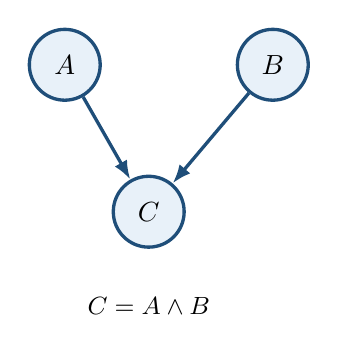
\begin{tikzpicture}[node distance=12mm and 17mm]
  \node[var] (a) {$A$};
  \node[var,right=of a] (b) {$B$};
  \node[var,below right=12mm and 4mm of a] (c) {$C$};
  \draw[flow] (a) -- (c);
  \draw[flow] (b) -- (c);
  \node[smalllabel,below=5mm of c] {$C=A\land B$};
\end{tikzpicture}

\scriptsize\path{m13_bucket3_binary_collider_and}
\end{minipage}\hfill
\begin{minipage}[t]{0.32\textwidth}
\centering
\textbf{H2: trailing distractor}

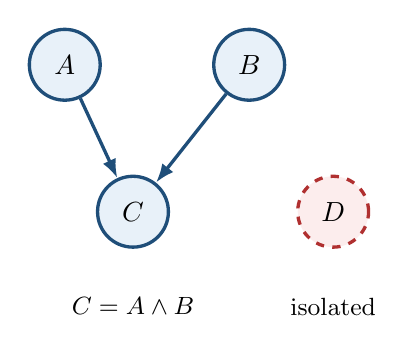
\begin{tikzpicture}[node distance=12mm and 14mm]
  \node[var] (a) {$A$};
  \node[var,right=of a] (b) {$B$};
  \node[var,below right=12mm and 2mm of a] (c) {$C$};
  \node[irrelevant,right=16mm of c] (d) {$D$};
  \draw[flow] (a) -- (c);
  \draw[flow] (b) -- (c);
  \node[smalllabel,below=5mm of c] {$C=A\land B$};
  \node[smalllabel,below=5mm of d] {isolated};
\end{tikzpicture}

\small target \(C\) BK order: \(A,B,D\)
\end{minipage}\hfill
\begin{minipage}[t]{0.32\textwidth}
\centering
\textbf{H3: leading distractor}

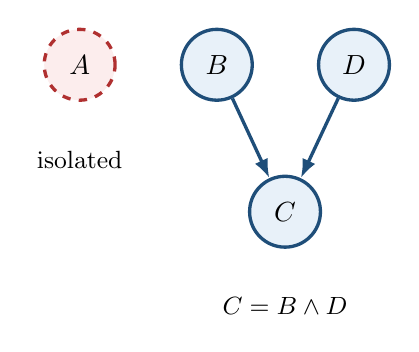
\begin{tikzpicture}[node distance=12mm and 14mm]
  \node[irrelevant] (a) {$A$};
  \node[var,right=8mm of a] (b) {$B$};
  \node[var,right=8mm of b] (d) {$D$};
  \node[var,below right=12mm and 2mm of b] (c) {$C$};
  \draw[flow] (b) -- (c);
  \draw[flow] (d) -- (c);
  \node[smalllabel,below=5mm of c] {$C=B\land D$};
  \node[smalllabel,below=5mm of a] {isolated};
\end{tikzpicture}

\small target \(C\) BK order: \(A,B,D\)
\end{minipage}
\caption{Controlled fixtures. Dashed red nodes are independent isolated
distractors. H2 tests a trailing distractor; H3 puts the distractor first in
the target-\(c\) BK.}
\label{fig:fixtures}
\end{figure}

The root probabilities are \(P(A=1)=0.8\), \(P(B=1)=0.7\) in H0/H2, with
\(D\sim\mathrm{Bernoulli}(0.5)\) in H2. H3 uses isolated
\(A\sim\mathrm{Bernoulli}(0.5)\), \(P(B=1)=0.8\), \(P(D=1)=0.7\), and
\(C=B\land D\). The principal samples are frozen \(n=30\), seed 42.

\subsection{What counts as a desirable solution}

Only deterministic child \(C\) has an evaluator mechanism over observed
parents. H0/H2 use

\begin{lstlisting}
c(A) :- a_val_1(A), b_val_1(A).
\end{lstlisting}

H3 uses

\begin{lstlisting}
c(A) :- b_val_1(A), d_val_1(A).
\end{lstlisting}

The roots and isolated variables have evaluator status
\code{no_observed_parent_deterministic_rule}. Their target-wise runs are
diagnostics: a procedural solution is not desirable merely because it covers
the sample.

\subsection{Compared learner bundles}

\begin{center}
\small
\begin{tabularx}{\textwidth}{>{\raggedright\arraybackslash}p{0.22\textwidth}
>{\raggedright\arraybackslash}p{0.13\textwidth}
>{\raggedright\arraybackslash}p{0.13\textwidth}X}
\toprule
Identity & Semantics & Folding & Other relevant options \\
\midrule
\code{aamas2025} & brave & greedy & mgr selection, BK folding space,
\code{relto} \\
\code{ecai2024} & brave & nd & any selection, all folding space,
steps 10, \code{relto} \\
\code{baseline_cautious} & cautious & nd & same nd baseline options,
steps 10, \code{relto} \\
H6 configurations & cautious & nd & baseline with steps \(1,2,5\), or 10 \\
\code{nd_brave_sechk} & brave & nd & H7a assumption-policy contrast \\
\bottomrule
\end{tabularx}
\end{center}

\section{Finding 1: Greedy retains every available predictor}

\finding
Under the complete-row exact-value encoding used in H0--H3, every completed
Greedy solution cites every non-target predictor variable in each learned
target rule. This includes predictors that are evaluator-known to be isolated
and irrelevant to the target mechanism. The successful deltas contain no final
assumptions or contraries.

\subsection{Comparison and observed evidence}

The strongest controlled evidence is H2/H3 target \(c\): the same kind of
isolated variable is placed last or first in BK, while Greedy retains it in
both cases.

\begin{figure}[ht]
\centering
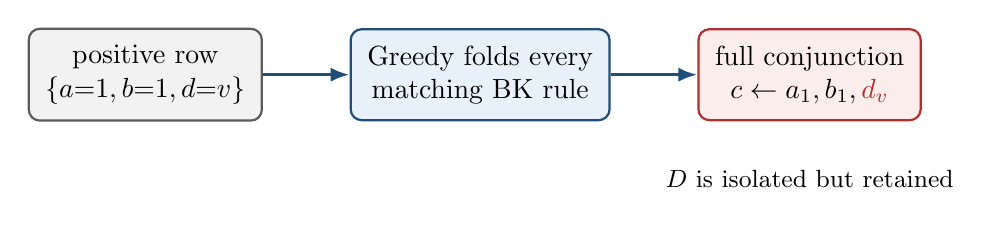
\begin{tikzpicture}[node distance=9mm and 11mm]
  \node[neutralbox] (row) {positive row\\
  \(\{a{=}1,b{=}1,d{=}v\}\)};
  \node[process,right=of row] (fold) {Greedy folds every\\matching BK rule};
  \node[warningbox,right=of fold] (rule) {full conjunction\\
  \(c\leftarrow a_1,b_1,\color{warningred}{d_v}\)};
  \draw[flow] (row) -- (fold);
  \draw[flow] (fold) -- (rule);
  \node[smalllabel,below=5mm of rule] {\(D\) is isolated but retained};
\end{tikzpicture}
\caption{Greedy exact-value folding converts the row identifier into all
matching predictor-value heads. It does not test whether the isolated
predictor is needed by the mechanism.}
\label{fig:greedy-full}
\end{figure}

\begin{center}
\small
\begin{tabularx}{\textwidth}{>{\raggedright\arraybackslash}p{0.12\textwidth}
>{\raggedright\arraybackslash}p{0.17\textwidth}
>{\raggedright\arraybackslash}p{0.15\textwidth}
>{\raggedright\arraybackslash}p{0.18\textwidth}X}
\toprule
Probe & Sample/target & Predictors in BK & Variables in every target-rule body & Reading \\
\midrule
H0 & \(n=30,c\) & \(a,b\) & \(a,b\) & Direct AND conjunction. \\
H1 & \(n=25,a\) & \(b,c\) & \(b,c\) & Spurious root rules. \\
H1 & \(n=25,b\) & \(a,c\) & \(a,c\) & Mirror spurious roots. \\
H1 & \(n=25,c\) & \(a,b\) & \(a,b\) & Direct AND conjunction. \\
H2 & \(n=30,c\) & \(a,b,d\) & \(a,b,d\) & Trailing isolated \(d\) retained. \\
H2c & \(n=2,b\) & \(a,c,d\) & \(a,c,d\) & Small-prefix solution. \\
H2c & \(n=2,c\) & \(a,b,d\) & \(a,b,d\) & Isolated \(d\) retained. \\
H3 & \(n=30,c\) & \(a,b,d\) & \(a,b,d\) & Leading isolated \(a\) retained. \\
\bottomrule
\end{tabularx}
\end{center}

H2 emits

\begin{lstlisting}
c(A) :- a_val_1(A), b_val_1(A), d_val_1(A).
c(A) :- a_val_1(A), b_val_1(A), d_val_0(A).
\end{lstlisting}

although the evaluator rule contains no \(d\). H3 emits

\begin{lstlisting}
c(A) :- a_val_1(A), b_val_1(A), d_val_1(A).
c(A) :- a_val_0(A), b_val_1(A), d_val_1(A).
\end{lstlisting}

although \(a\) is isolated. H5 duplicates all five completed AAMAS collections
under experimental Greedy-cautious learning: all 18 outcomes match and every
solved delta is byte-identical. Across these solved deltas, the number of final
assumptions and contraries is zero.

\explanation
Rote learning initially distinguishes rows by identifier. With
\code{folding_mode(greedy)} and \code{folding_space(bk)}, the Greedy fold walks
the row-specific body and accumulates every eligible BK head that matches the
row. Complete exact-value BK supplies one matching value predicate for every
non-target column. The resulting full conjunction usually already separates
the finite examples, so \code{gen2} accepts it without assumption introduction.
There is no later literal-deletion, cross-rule anti-unification, or mechanism
minimality stage that can remove an irrelevant column.

\implication
Greedy is a poor fit when the scientific objective is \emph{minimal
mechanism-variable selection} under this exact-value encoding. Its full-row
specialisation systematically preserves distractors. This supports using nd
or another constrained search when selective bodies are required.

\boundary
The evidence does not establish that Greedy is globally inferior to nd. Nd has
its own first-variable and assumption-gadget failures, and Greedy is much
cheaper on these fixtures. Nor is full-variable citation a theorem for every
possible ABA BK: it is the stable result of the tested complete exact-value
representation and configuration. Greedy can attempt assumptions when a fold
fails; several no-solution traces do so. The claim here concerns its
\emph{completed solutions} in scope.

\section{Finding 2: nd solutions are anchored to the first BK predictor}

\finding
Across the completed solved nd cells inspected in H0/H3 and their H4/H4b/H6/H7
ablations, the first predictor in target-specific BK appears in the final
target theory. H3 proves that this need not be causally or mechanistically
relevant: isolated \(A\) is first in the target-\(c\) BK and becomes the outer
gate of the learned theory.

\subsection{Comparison and observed evidence}

H3 fixes \(C=B\land D\), introduces isolated \(A\), and orders the target-\(c\)
predictors as \(A,B,D\). Under brave nd/\code{relto}, the first fold is:

\begin{lstlisting}
folding result: c(A) <- [a_val_1(A)]
\end{lstlisting}

and the final ordinary target rules are:

\begin{lstlisting}
c(A) :- alpha_1(A), a_val_1(A).
c(A) :- alpha_2(A), a_val_0(A).
\end{lstlisting}

\begin{figure}[ht]
\centering
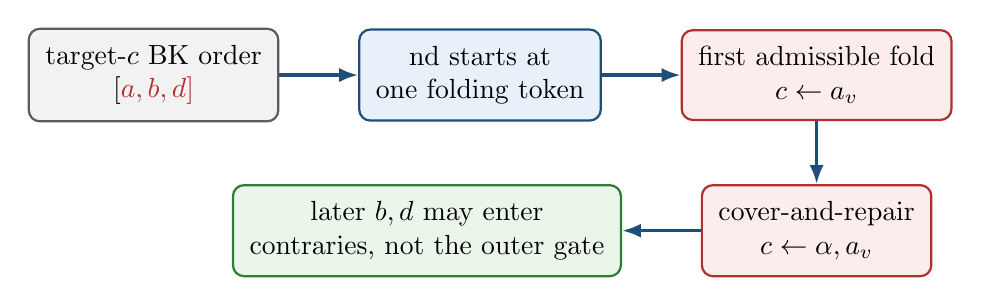
\begin{tikzpicture}[node distance=8mm and 10mm]
  \node[neutralbox] (order) {target-\(c\) BK order\\
  \([\color{warningred}{a},b,d]\)};
  \node[process,right=of order] (token) {nd starts at\\one folding token};
  \node[warningbox,right=of token] (first) {first admissible fold\\
  \(c\leftarrow a_v\)};
  \node[warningbox,below=of first] (gate) {cover-and-repair\\
  \(c\leftarrow\alpha,a_v\)};
  \node[evidencebox,left=of gate] (later) {later \(b,d\) may enter\\contraries,
  not the outer gate};
  \draw[flow] (order) -- (token);
  \draw[flow] (token) -- (first);
  \draw[flow] (first) -- (gate);
  \draw[flow] (gate) -- (later);
\end{tikzpicture}
\caption{First-fold commitment in H3. The isolated first predictor becomes
structural scaffolding for the learned ABA theory before mechanism parents are
considered.}
\label{fig:first-bk}
\end{figure}

H0 supplies the non-distractor counterpart: for target \(c\), BK order
\([a,b]\) gives an \(a\)-gated target rule; for target \(a\), order \([b,c]\)
gives \(b\)-gated rules. H7a broadens the observation across both fixtures:
all seven brave-nd \code{sechk} deltas cite exactly the first predictor and no
later observed variable, whereas the \code{relto} comparator can introduce
later variables into contraries after a failed reuse. H4b and H7b show that
cautious semantics changes later repairs, but the leading-\(a\) outer gates on
the H3 child remain.

\explanation
Nd begins with one folding token and the \code{any} selection policy. Given the
serialized BK order, the first admissible value literal is tried first. If the
unary fold overgeneralises, the learner's cover-and-repair machinery adds an
assumption rather than reconsidering the scientific relevance of the initial
predictor. Later variables can repair contraries, but the first literal remains
in the ordinary target rule. H7a's \code{sechk} path makes the preference more
extreme: it mints an assumption immediately and, on those brave traces, closes
an assumption chain before reaching later predictors.

\implication
BK order is a scientifically consequential search intervention. A later
integration could use independently justified information---for example,
dependence screening, conditional-independence evidence, or Causal ABA
constraints---to rank which predicates nd considers first. The aim would be
to make early folds more plausible, not to expose the evaluator DAG or target
mechanism directly to the learner.

\boundary
The experiments establish order sensitivity and persistent first-predictor
inclusion, not that correlation provides the correct causal ordering or that a
Causal-ABA-guided order improves recovery. Correlation may favour descendants,
siblings, or proxies. This implication is therefore a concrete integration
hypothesis requiring a controlled reordering experiment. ``Always'' is bounded
to the solved nd cells and configurations inspected, not an algorithmic law
for arbitrary BK.

\section{Finding 3: brave nd can report a non-functional root solution}

\finding
On H0, brave nd reports \code{solved} for roots \(a\) and \(b\), although each
root is stochastic and has no deterministic evaluator rule over the other
observed variables. The solution uses grounded assumptions to distinguish rows
whose learner-visible predictors are identical. Cautious nd rejects the
decisive residual reuse and returns \code{completed_no_solution} for both roots
through folding budget 10, while still solving child \(c\).

\subsection{The 9/26 information conflict}

For target \(a\), the learner receives \(b,c\) as predictors. Rows 9 and 26
have identical predictor values but opposite target labels:

\begin{center}
\begin{tabular}{ccccc}
\toprule
Row & \(A\) (target) & \(B\) & \(C\) & Example \\
\midrule
9  & 1 & 0 & 0 & \(a(9)\in\Epos\) \\
26 & 0 & 0 & 0 & \(a(26)\in\Eneg\) \\
\bottomrule
\end{tabular}
\end{center}

No deterministic function \(f(B,C)\) can satisfy both
\(f(0,0)=1\) and \(f(0,0)=0\).

\begin{figure}[ht]
\centering
\resizebox{0.98\textwidth}{!}{%
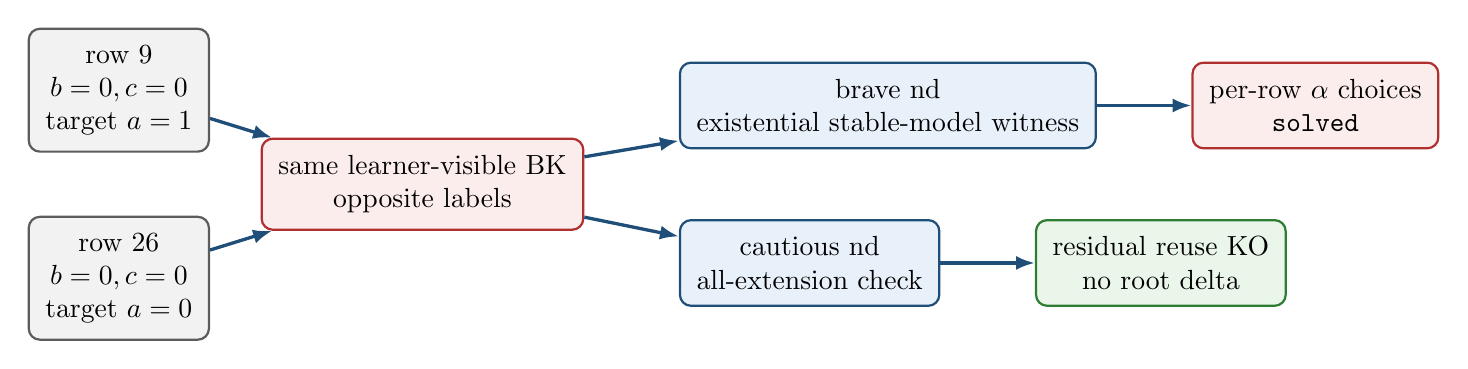
\begin{tikzpicture}[node distance=8mm and 12mm]
  \node[neutralbox] (r9) {row 9\\\(b=0,c=0\)\\target \(a=1\)};
  \node[neutralbox,below=of r9] (r26) {row 26\\\(b=0,c=0\)\\target \(a=0\)};
  \node[warningbox,right=18mm of $(r9)!0.5!(r26)$] (conflict)
    {same learner-visible BK\\opposite labels};
  \node[process,right=of conflict,yshift=10mm] (brave)
    {brave nd\\existential stable-model witness};
  \node[warningbox,right=of brave] (bsolve)
    {per-row \(\alpha\) choices\\\code{solved}};
  \node[process,right=of conflict,yshift=-10mm] (cautious)
    {cautious nd\\all-extension check};
  \node[evidencebox,right=of cautious] (cnosol)
    {residual reuse KO\\no root delta};
  \draw[flow] (r9) -- (conflict);
  \draw[flow] (r26) -- (conflict);
  \draw[flow] (conflict) -- (brave);
  \draw[flow] (brave) -- (bsolve);
  \draw[flow] (conflict) -- (cautious);
  \draw[flow] (cautious) -- (cnosol);
\end{tikzpicture}
}
\caption{The 9/26 conflict and the semantic fork. The rows cannot be separated
by \(b,c\); brave nd nevertheless constructs a grounded assumption witness.}
\label{fig:nine-twentysix}
\end{figure}

\subsection{Brave construction and cautious rejection}

The relevant brave block is:

\begin{lstlisting}
a(A) :- alpha_2(A), b_val_0(A).
c_alpha_2(A) :- alpha_3(A), c_val_0(A).
c_alpha_3(A) :- alpha_2(A), b_val_0(A).
\end{lstlisting}

with assumptions and contrary declarations for \(\alpha_2,\alpha_3\). Because
the assumptions are grounded by row identifier, a witnessing stable extension
can accept the appropriate assumption instances at row 9 and defeat them at
row 26. The framework covers the sample under brave entailment without making
\(A\) a function of \(B,C\).

The decisive traces differ at the same proposed reuse:

\begin{center}
\small
\begin{tabularx}{\textwidth}{>{\raggedright\arraybackslash}p{0.17\textwidth}
>{\raggedright\arraybackslash}p{0.39\textwidth}X}
\toprule
Mode & Trace decision & Outcome for root \(a\) \\
\midrule
Brave nd & \code{found: alpha_2/1 ... OK} for
\code{c_alpha_3 <- [alpha_2,b_val_0]} & \code{solved}; 11-rule
assumption framework \\
Cautious nd & \code{found: alpha_2/1 ... KO} for the same residual reuse &
Further backtracking and token retries; \code{completed_no_solution} at
steps 10 \\
\bottomrule
\end{tabularx}
\end{center}

The mirror result holds for target \(b\). The child \(c\) is an important
control: both modes solve it and emit byte-identical deltas. Cautious learning
does not merely suppress all outputs; it blocks this particular non-functional
root construction.

\explanation
Brave entailment needs a suitable stable extension witnessing the joint
example constraints. Ground assumption instances can therefore behave
differently for different row identifiers. Cautious checking rejects the
residual rule because its acceptance is not stable across the relevant
extensions. The search then explores further nd folds, but no accepted root
theory appears within the permitted budget.

\implication
If the evaluation objective is to avoid reporting existential, per-row choice
frameworks as recovered predictor-to-target rules, cautious semantics is the
better nd baseline for the next integration stage. It preserves the useful
child control while refusing the H0 root gadget.

\boundary
This is not a proof that cautious nd can never produce a misleading solution,
nor that every brave solution is misleading. The result is fixed to H0,
\code{relto}, and the tested budget through 10. Cautious
\code{completed_no_solution} is a guardrail/non-result, not recovery of a root
mechanism. It is also computationally much more expensive here.

\section{Finding 4: cautious-nd failure cost scales with folding budget}

\finding
At fixed H0 \(n=30\), cautious-nd root trace length is approximately linear in
the permitted \code{folding_steps} ceiling \(M\in\{1,2,5,10\}\). Every root
run remains \code{completed_no_solution}; child \(c\) solves within token
budget 1 and is unaffected by a larger ceiling.

\subsection{H6a design and result}

\begin{center}
\small
\begin{tabular}{rrrrr}
\toprule
\(M\) & target \(a\) lines & runtime (s) & NEW assumptions & KO \\
\midrule
1  & 549  & 6.638  & 9  & 16 \\
2  & 1047 & 13.117 & 18 & 32 \\
5  & 2541 & 32.775 & 45 & 80 \\
10 & 5031 & 69.952 & 90 & 160 \\
\bottomrule
\end{tabular}
\end{center}

Target \(b\) mirrors the pattern. At every \(M\), target \(c\) has the same
134-line trace, approximately 1.3-second runtime, and byte-identical delta.

\begin{figure}[ht]
\centering
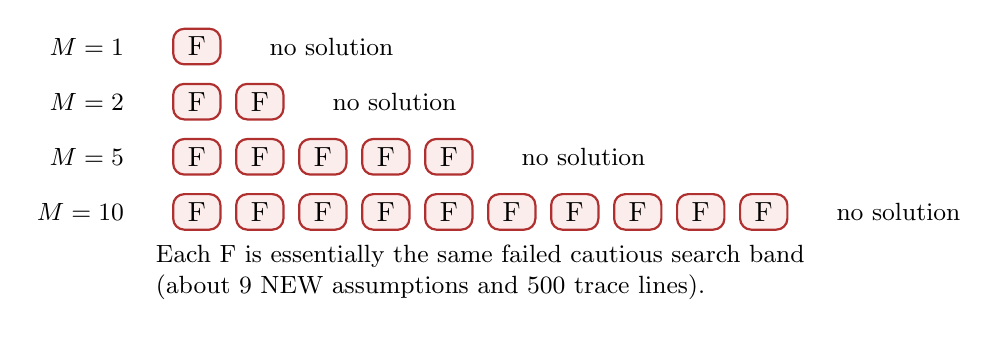
\begin{tikzpicture}[x=8mm,y=7mm]
  \node[smalllabel,anchor=east] at (0,0) {\(M=1\)};
  \node[smalllabel,anchor=east] at (0,-1) {\(M=2\)};
  \node[smalllabel,anchor=east] at (0,-2) {\(M=5\)};
  \node[smalllabel,anchor=east] at (0,-3) {\(M=10\)};
  \foreach \x in {1} {\node[warningbox,minimum width=6mm,inner sep=3pt] at (\x,0) {F};}
  \foreach \x in {1,2} {\node[warningbox,minimum width=6mm,inner sep=3pt] at (\x,-1) {F};}
  \foreach \x in {1,2,3,4,5} {\node[warningbox,minimum width=6mm,inner sep=3pt] at (\x,-2) {F};}
  \foreach \x in {1,2,3,4,5,6,7,8,9,10}
    {\node[warningbox,minimum width=6mm,inner sep=3pt] at (\x,-3) {F};}
  \node[smalllabel,anchor=west] at (2.0,0) {no solution};
  \node[smalllabel,anchor=west] at (3.0,-1) {no solution};
  \node[smalllabel,anchor=west] at (6.0,-2) {no solution};
  \node[smalllabel,anchor=west] at (11.0,-3) {no solution};
  \node[smalllabel,align=left] at (5.5,-4.1)
    {Each F is essentially the same failed cautious search band\\
     (about 9 NEW assumptions and 500 trace lines).};
\end{tikzpicture}
\caption{H6a mechanism: \(M\) is a token-budget ceiling. On these roots, a
higher ceiling replays a failed motif instead of extending one continuous
successful derivation.}
\label{fig:budget-bands}
\end{figure}

\explanation
Under nd, the learner starts at \code{tokens(1)}. If the entire search under
that allowance fails, \code{genT} increments the token allowance and restarts
while \(T+1\leq M\). On H0 roots, the decisive cautious KO already appears in
the first band. Each extra band reconstructs essentially the same nine-new-
assumption pattern at a higher printed fold counter. Empirically,

\[
  \operatorname{lines}(M)\approx C_{\mathrm{fixed}}+M C_{\mathrm{failed\ band}},
  \qquad C_{\mathrm{failed\ band}}\approx 500\text{ lines}.
\]

The sequence NEW \(=9,18,45,90\) is exactly \(9M\). The extra budget through
\(M=10\) does not change the outcome or produce a candidate delta.

\implication
The maximum folding allowance should be an explicit, input-sensitive resource
decision rather than an unexplained constant of 10. A practical integration
could use a low initial ceiling and stop when higher-token bands reproduce the
same conflicts without new accepted structure. Causal or functional
pre-analysis might also identify targets for which large search is unlikely to
be useful.

\boundary
H6a does not derive a universal input-to-budget formula or show that \(M=1\)
is always sufficient. Some learnable targets may require more folding tokens.
The defensible result is narrower: on the tested no-solution roots, \(M=10\)
spent roughly ten failed bands, while the learnable child finished at token 1.
An adaptive stopping rule remains to be designed and tested.

\section{Finding 5: cautious-nd trace size scales with grounded sample size}

\finding
At fixed folding ceiling \(M=2\), cautious-nd trace length grows approximately
linearly with nested sample size \(n\in\{30,60,90\}\). H0 population support is
already fully represented at \(n=30\); the larger tables add multiplicities and
ground row identifiers, not new joint value patterns. Root outcomes and search
topology remain unchanged.

\subsection{H6b design and result}

\begin{figure}[ht]
\centering
\resizebox{0.96\textwidth}{!}{%
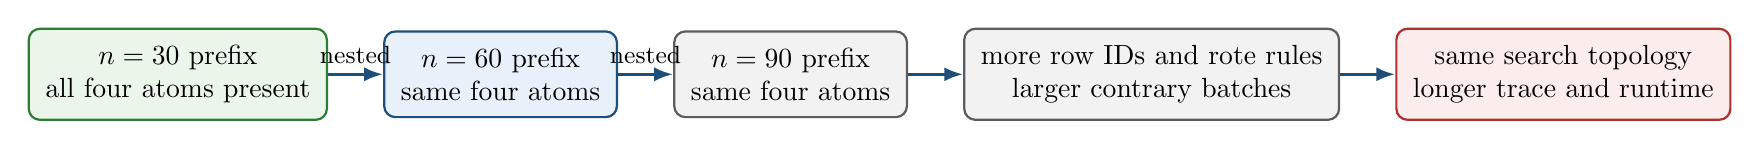
\begin{tikzpicture}[node distance=7mm]
  \node[evidencebox] (n30) {\(n=30\) prefix\\all four atoms present};
  \node[process,right=of n30] (n60) {\(n=60\) prefix\\same four atoms};
  \node[neutralbox,right=of n60] (n90) {\(n=90\) prefix\\same four atoms};
  \node[neutralbox,right=of n90] (ground)
    {more row IDs and rote rules\\larger contrary batches};
  \node[warningbox,right=of ground] (cost)
    {same search topology\\longer trace and runtime};
  \draw[flow] (n30) -- node[above,smalllabel] {nested} (n60);
  \draw[flow] (n60) -- node[above,smalllabel] {nested} (n90);
  \draw[flow] (n90) -- (ground);
  \draw[flow] (ground) -- (cost);
\end{tikzpicture}
}
\caption{H6b mechanism. The nested prefixes preserve support presence from
\(n=30\), while multiplicity increases the grounded bookkeeping performed in
each fixed search band.}
\label{fig:n-scaling}
\end{figure}

\begin{center}
\small
\begin{tabular}{rrrrrr}
\toprule
\(n\) & target \(a\) lines & runtime (s) & NEW & KO & target \(c\) lines \\
\midrule
30 & 1047 & 13.117 & 18 & 32 & 134 \\
60 & 1641 & 22.169 & 18 & 32 & 200 \\
90 & 2241 & 32.291 & 18 & 32 & 266 \\
\bottomrule
\end{tabular}
\end{center}

For target \(a\), line increments are \(+594\) and \(+600\) for each additional
30 rows. Target \(b\) mirrors this. Target \(c\) retains a byte-identical delta
while its trace grows by 66 lines per 30 rows.

The four atom counts, ordered as
\((0,0,0),(0,1,0),(1,0,0),(1,1,1)\), are:

\[
  n=30: (2,4,7,17),\qquad
  n=60: (4,10,12,34),\qquad
  n=90: (5,17,18,50).
\]

\explanation
At fixed \(M=2\), root traces have the same procedural topology: 18 NEW
assumptions, 32 KOs, and one token increase. More rows enlarge the ground
\(\Epos/\Eneg\) sets, row-specific rote rules, entailment checks, subsumption
sweeps, and contrary batches within each band. Consequently, trace lines grow
roughly in proportion to \(n\) over this tested range. Runtime grows slightly
faster because ASP consequence checks are not constant-cost per printed line.

\implication
The present learner does not use empirical frequencies as statistical weights;
duplicate value patterns chiefly create additional grounded examples. A
promising later pipeline is therefore:

\begin{figure}[ht]
\centering
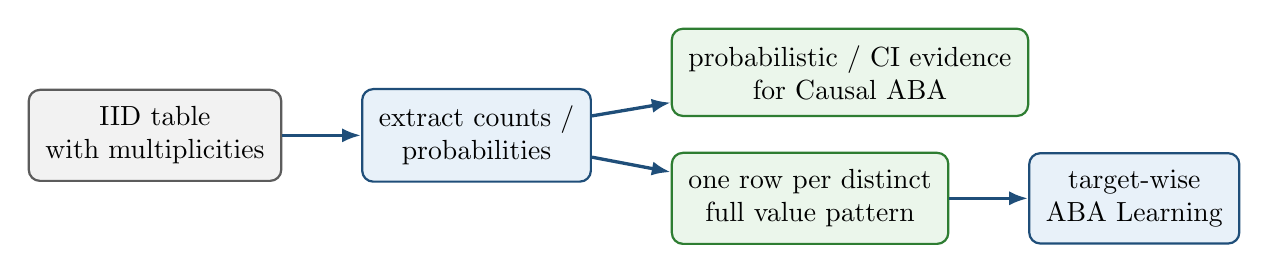
\begin{tikzpicture}[node distance=8mm and 10mm]
  \node[neutralbox] (table) {IID table\\with multiplicities};
  \node[process,right=of table] (extract) {extract counts /\\probabilities};
  \node[evidencebox,right=of extract,yshift=8mm] (causal)
    {probabilistic / CI evidence\\for Causal ABA};
  \node[evidencebox,right=of extract,yshift=-8mm] (unique)
    {one row per distinct\\full value pattern};
  \node[process,right=of unique] (learn) {target-wise\\ABA Learning};
  \draw[flow] (table) -- (extract);
  \draw[flow] (extract) -- (causal);
  \draw[flow] (extract) -- (unique);
  \draw[flow] (unique) -- (learn);
\end{tikzpicture}
\caption{Proposed, not yet tested: preserve frequency information in a
probabilistic causal layer while giving the symbolic learner a support-compressed
table.}
\label{fig:dedup-proposal}
\end{figure}

Once counts or probabilities have been extracted and preserved separately for
the causal component, passing only unique full rows to ABA Learning could avoid
redundant grounding while retaining the observed support and predictor-label
conflicts relevant to deterministic-rule learning.

\boundary
H6b is a nested-\(n\) experiment, not a direct deduplication ablation. The
larger prefixes change empirical frequencies, and duplicate removal can alter
row order, selection, or learner behaviour even when logical support is
unchanged. Therefore ``duplicates add no benefit'' is a proposed engineering
hypothesis conditional on preserving their probabilistic information elsewhere.
It should be verified by comparing a frozen full table with a support-compressed
counterpart before adoption. The observed linearity is local, not a universal
complexity law.

\section{What the five findings jointly support}

\begin{longtable}{>{\raggedright\arraybackslash}p{0.20\textwidth}
>{\raggedright\arraybackslash}p{0.34\textwidth}
>{\raggedright\arraybackslash}p{0.36\textwidth}}
\toprule
Area & Directly supported statement & Proposed decision for discussion \\
\midrule
\endhead
Greedy & Complete exact-value Greedy solutions in scope cite every predictor;
isolated variables survive. & Avoid Greedy when minimal mechanism-variable
selection is the primary objective; do not infer that nd is globally superior. \\
\addlinespace
Nd order & The first BK predictor occurs in every solved nd theory inspected;
H3 shows it can be isolated. & Investigate causally or statistically informed
BK ordering as a controlled integration, with leakage and confounding checks. \\
\addlinespace
Semantics & Brave nd solves H0 roots through a per-row assumption gadget;
cautious nd rejects the decisive reuse and emits no root delta through \(M=10\). &
Use cautious nd as the safer baseline when a recovered rule should not depend on
an existential row-wise choice. \\
\addlinespace
Folding budget & H0 no-solution root cost grows by replaying approximately one
failed band per permitted token. & Replace an arbitrary ceiling of 10 with an
explicit resource policy or novelty-based early stopping. \\
\addlinespace
Sample size & At fixed topology, trace size grows roughly with grounded \(n\)
after all population atoms are already present. & Test support compression after
probabilistic information has been extracted and retained separately. \\
\bottomrule
\end{longtable}

These five results favour a division of labour in a future integration:

\begin{enumerate}
  \item a statistical/causal layer extracts frequency, dependence, and graph-
  compatibility information;
  \item that information guides representation, BK ordering, and search
  resources without exposing evaluator ground truth;
  \item cautious target-wise ABA Learning produces inspectable rules and
  exception structures over a compact support representation; and
  \item evaluation checks functional adequacy, minimality, invariance, and
  causal compatibility separately from the procedural \code{solved} label.
\end{enumerate}

This is a research programme motivated by H0--H7b, not a completed Causal ABA
integration or a demonstrated graph-discovery algorithm.

\appendix

\section{Evidence map}

All qualitative records below are relative to:

\begin{lstlisting}
docs/experiments/qualitative/M13-C3-binary-collider-and/
\end{lstlisting}

\begin{longtable}{>{\raggedright\arraybackslash}p{0.11\textwidth}
>{\raggedright\arraybackslash}p{0.35\textwidth}
>{\raggedright\arraybackslash}p{0.43\textwidth}}
\toprule
Finding & Primary records & Principal learner artefacts \\
\midrule
\endhead
1 & \path{learning_analysis.md}; \path{h1_support_ablation.md};
\path{h2_irrelevant_covariate.md}; \path{h3_bk_leading_distractor.md};
\path{h5_greedy_cautious.md} & AAMAS and \code{greedy_cautious}
\path{delta.aba} files under the H0/H1/H2/H2c/H3 collections. \\
\addlinespace
2 & \path{h3_bk_leading_distractor.md};
\path{h7a_relto_vs_sechk.md}; \path{h4b_cautious_split_under_a.md};
\path{h7b_cautious_relto_vs_sechk.md} & H3 target-\(c\)
\path{ecai2024/n30_seed42}; H7a \path{nd_brave_sechk/n30_seed42};
H7b \path{nd_cautious_sechk/n30_seed42}. \\
\addlinespace
3 & \path{learning_analysis.md}; \path{h4_cautious_vs_brave.md} & H0
target-\(a,b,c\) collections under \path{ecai2024/n30_seed42} and
\path{baseline_cautious/n30_seed42}; especially target-\(a\)
\path{output/prolog.stdout} and brave \path{delta.aba}. \\
\addlinespace
4 & \path{h6_folding_and_n_ablation.md} & H0 \(n=30\) collections under
\path{baseline_cautious_steps1}, \path{baseline_cautious_steps2},
\path{baseline_cautious_steps5}, and reused steps-10
\path{baseline_cautious}. \\
\addlinespace
5 & \path{h6_folding_and_n_ablation.md} & H0
\path{baseline_cautious_steps2} collections for
\path{n30_seed42}, \path{n60_seed42}, and \path{n90_seed42}. \\
\bottomrule
\end{longtable}

Fixture specifications:

\begin{itemize}
  \item \path{causal/fixtures/specs/m13_bucket3_binary_collider_and.yaml};
  \item \path{causal/fixtures/specs/m13_bucket3_binary_collider_and_iso_d.yaml};
  \item \path{causal/fixtures/specs/m13_bucket3_binary_bd_and_lead_a.yaml}.
\end{itemize}

Implementation points used only to explain recorded behaviour:

\begin{itemize}
  \item \path{folding.pl}: \code{fold_greedy/3} and nd folding;
  \item \path{gen.pl}: post-fold entailment, assumption introduction, and the
  nd token-increase loop;
  \item \path{configs/aamas2025_config.pl};
  \item \path{configs/ecai2024_config.pl};
  \item \path{configs/baseline_cautious_config.pl}.
\end{itemize}

\section{Claim-status reminder}

The canonical Bucket~3 hub still records no approved claim. The five statements
in this document are bounded candidate findings for supervisor discussion.
Any later report claim should be checked against the primary experiment record,
the exact serialized output, and the claims ledger. The recommendations on BK
guidance, adaptive budgets, and support compression are next-stage design
hypotheses, not results already validated by H0--H7b.

\end{document}
